\documentclass[../main.tex]{subfiles}

\begin{document}

\chapter{Hierarchical Clustering Model} \label{hierarchical_clustering_model}

% Quick overview of HCA again
% Distance metric

% Talk about maintaining "unsupervised" nature; build search space now evaluate next
% Criteria being varied in search space; linkage [4], number of sectors [15; range from 5-19]
% Visualize search space


In the previous chapter, we evaluated major families of learning methods and identified the Hierarchical Clustering Analysis (hereafter \textit{HCA}) algorithm to be the method best aligned with the research goals of the project. Here we outline the specifics of our approach to applying HCA to our model input data, and build a search space of candidate universes to be evaluated, fully addressing RG-1.

\section{HCA Overview}

As outlined in Section~\ref{learning_methods_survey:hca}, hierarchical clustering is a greedy learning algorithm which seeks to construct a hierarchy of clusters. The greedy nature of this algorithm results in extremely high computational complexity for any given model fit, but is extremely stable in its solution. Furthermore, it is an $\mathcal{O}(1)$ complexity operation to extract classifications of varying arity due to the persistent hierarchical nature of the algorithm.

One of the main requirements of our heuristic is the ability to create sector universes with varying numbers of sectors. Because of this, we elected to utilize an Agglomorative approach to clustering. That is, we utilize a \textit{bottom-up} HCA model, where each company begins in its own sector, with larger clusters derived at each successive step of the tree by merging existing pairs of clusters.

Any given HCA algorithm tree is parameterized by two distinct settings; the distance metric, and the linkage method. To best understand the potential candidate universes that may be generated by this HCA-driven classification heuristic, we analyzed each of these model settings in turn:

\subsection{Distance Metric}

The distance metric is the measure of the distance between pairs of observations. This setting primarily affects the shape of the clusters. Due to the fact that our model input data is exclusively in monetary units (i.e. United States Dollars), we do not intend to transform the existing metric of wealth reflected by the dollar value measurement. Thus, we chose to use the $\ell^2$ (i.e. Euclidean) distance metric for our heuristic.

\begin{gather*}
    \text{Let $\boldsymbol{p}, \boldsymbol{q}$} = \text{Cartesian coordinates $\boldsymbol{p} = (p_1, \ldots, p_n)$ and $\boldsymbol{q} = (q_1, \ldots, q_n)$ where $\{\boldsymbol{p}, \boldsymbol{q}\} \in \mathbb{R}^{n \times 2}$} \\
    \text{Let $dist(\boldsymbol{p},\boldsymbol{q})$} = \text{$\ell^2$ (i.e. Euclidean) distance between points $\boldsymbol{p}$ and $\boldsymbol{q}$} \\
    \\
    \Rightarrow dist(\boldsymbol{p}, \boldsymbol{q}) = dist(\boldsymbol{q}, \boldsymbol{p})
    = \sqrt{(p_1 - q_1)^2 + (p_2 - q_2)^2 + \cdots + (p_n - q_n)^2}
    = \sqrt{\sum_{i=1}^n (p_i - q_i)^2}
\end{gather*}

\subsection{Linkage Method}

The second setting governing the behavior of the HCA algorithm is the selection of a linkage method. The linkage is a measure of distance between sets of observations as a function of the pairwise distances between observations. There are four major linkage method choices that we evaluate in our HCA model:


    $$ \text{Let $A, B, C, X, Y$} = \text{Sets (i.e. clusters) of observations} $$
    $$ \text{Let $C$} = X \cup Y $$
    $$ \text{Let $N$} = |A| + |X| + |Y|, \; \text{where} \; |\alpha| = \text{Cardinality}(\alpha) $$
    
\hspace{7em} \textbf{Single Linkage\citeFormat{\cite{Sibson1973SLINK:Method}}:}
        $$ d_\text{SLINK}(A, B) = \text{min} \; dist(\boldsymbol{a}, \boldsymbol{b})  \; \forall \; \{ \boldsymbol{a}, \boldsymbol{b} : \boldsymbol{a} \in A, \boldsymbol{b} \in B \} $$
    
\hspace{7em} \textbf{Complete Linkage\citeFormat{\cite{Defays1977AnMethod}}:}
        $$ d_\text{CLINK}(A, B) = \text{max} \; dist(\boldsymbol{a}, \boldsymbol{b})  \; \forall \; \{ \boldsymbol{a}, \boldsymbol{b} : \boldsymbol{a} \in A, \boldsymbol{b} \in B \} $$
    
\hspace{7em} \textbf{Average Linkage\citeFormat{\cite{Seifoddini1989SingleApplications}}:}
        $$ d_\text{ALC}(A, B) = \frac{1}{|A| \cdot |B|} \sum_{\boldsymbol{a} \in A} \sum_{\boldsymbol{b} \in B} dist(\boldsymbol{a}, \boldsymbol{b}) $$
    
\hspace{7em} \textbf{Ward (variance minimization) Linkage\citeFormat{\cite{Ward1963HierarchicalFunction}}:}
        $$ d_\text{WARD}(C, A) = \sqrt{ \frac{|A| + |X|}{N} d_\text{WARD}(A, X)^2 + \frac{|A| + |Y|}{N} d_\text{WARD}(A, Y)^2 - \frac{|A|}{N} d_\text{WARD}(X, Y)^2 } $$

\section{Unsupervised Learning Approach}

\begin{wrapfigure}[14]{r}{0.45\textwidth}
    \centering
    \vspace{\wrapfigadjustment}
    \fbox{
    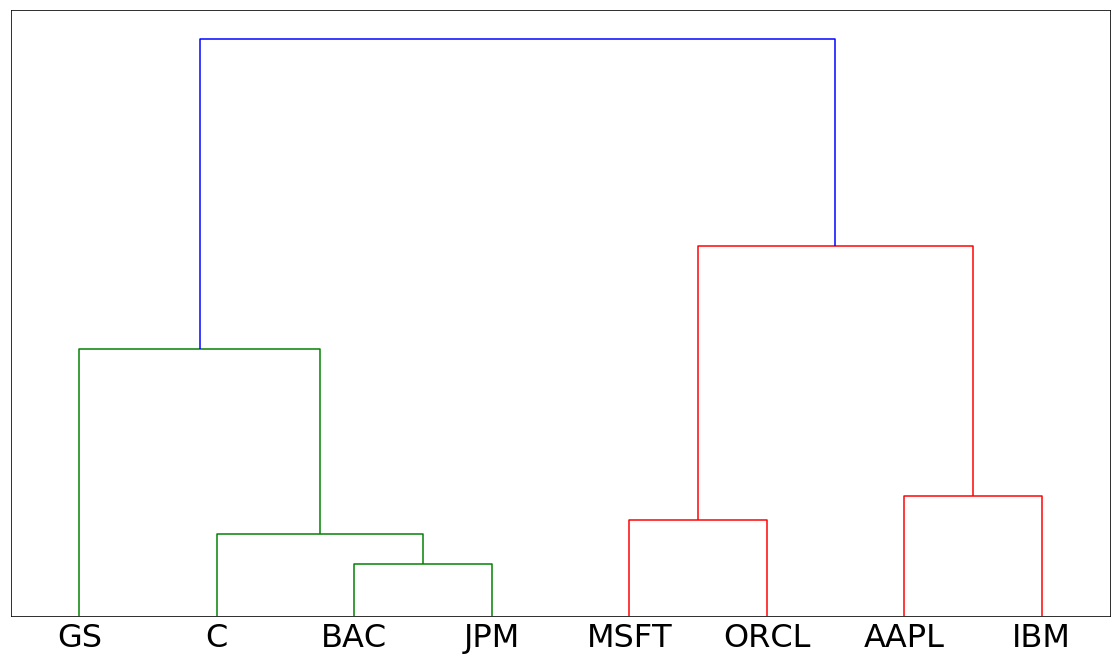
\includegraphics[width=.9\linewidth]{images/tree.png}
    }
    \caption{Dendrogram of a sample hierarchical clustering model result.}
    \label{fig:hierarchical_clustering_model:sample_dendogram}
\end{wrapfigure}

As per RG-1 (see Section~\ref{research_goals:specific_research_goals}), we seek to create an entirely objective classification heuristic. Logically, this implies that we utilize an entirely nonparametric approach when designing the classification heuristic. However, as discussed above, the HCA algorithm is parameterized by both the distance metric, and the linkage method (in addition to a posterior selection of the number of sectors).

To work around the semi-supervised nature of the learning method, we elected to utilize HCA to build a search space of potential candidate sector universes. Following this, we will address our second research goal, RG-2, to rank these candidate sector universes against each other to determine the optimal learned sector classification.

Note that this search-space generation varies the sector count and linkage method parameters of the HCA model, but not the distance metric. This is due to the fact that we wish to preserve the monotonic and geometric difference of magnitudes of wealth implied by the dollar values of our input data.

Figure~\ref{fig:hierarchical_clustering_model:sample_dendogram} is a dendrogram of a sample HCA model generated on a subset of the model input data. Despite having a very high time complexity for model training, the HCA model thrives in its ability to extract sector classifications of varying arity from a HCA model. Its ability to perform this action in constant time complexity greatly enhanced our ability to generate a large search space of candidate learned sector universes.


\pagebreak

\section{Learned Sector Universe Search Space}


\begin{figure}[h]
    \centering
    \fbox{
    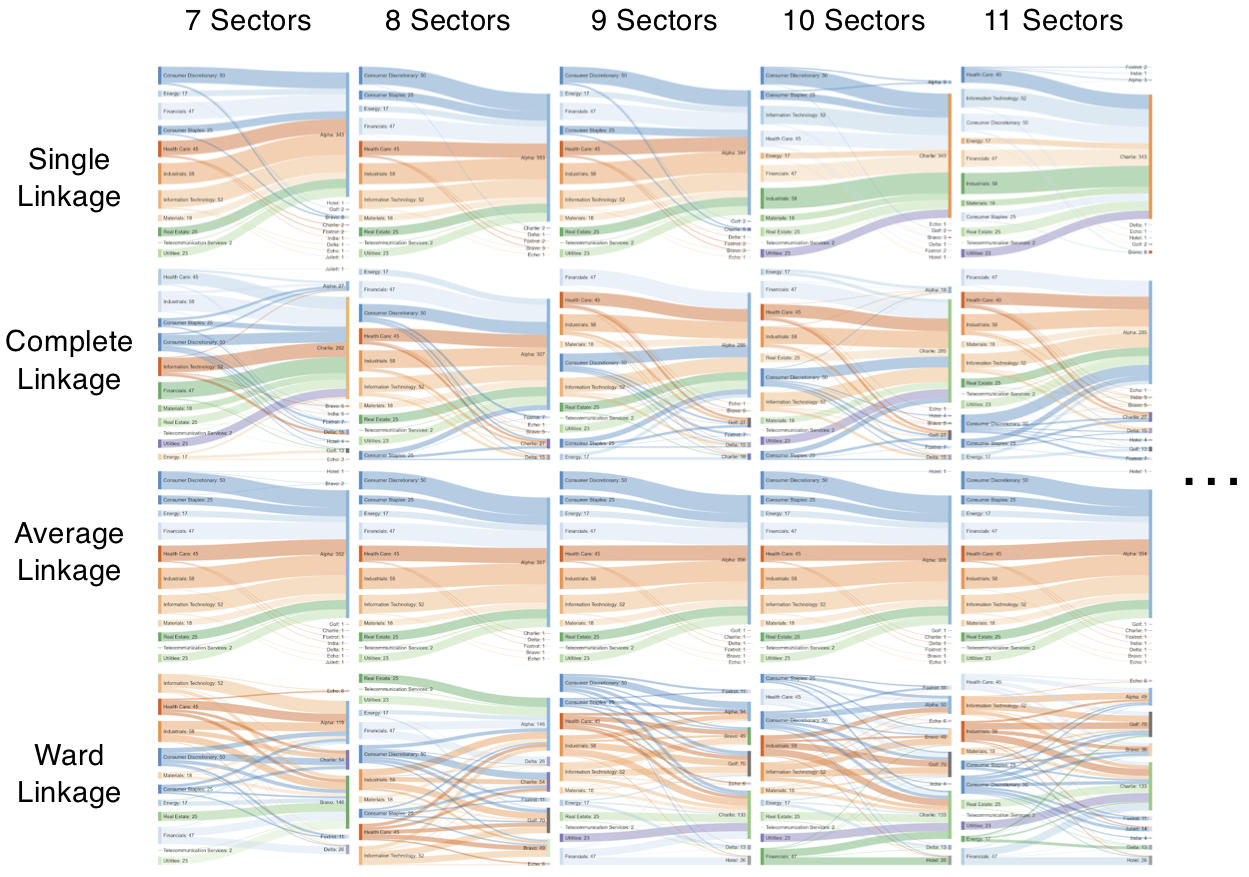
\includegraphics[width=.8\linewidth]{images/search_space_partial.png}
    }
    \caption{Candidate learned sectors partial search space visualization.}
    \label{fig:hierarchical_clustering_model:partial_search_space}
\end{figure}

With the end goal of building a comprehensive search space of candidate learned sector classifications, we generated HCA models parameterized with each of the linkage methods, and then isolated sector classifications for varying numbers of sectors. Specifically, we varied the number of sectors in our search space universes with $N = \{5, 6, \ldots, 19 \}$ for each of the four linkage methods, for a total of 60 candidate learned sector universes. A subset of our search space is visualized in Figure~\ref{fig:hierarchical_clustering_model:partial_search_space}.

The HCA models were generated iteratively using the model input data discussed in Section~\ref{model_data}. We utilized the built-in Hierarchical Clustering Module in \textit{Scikit-learn}\citeFormat{\cite{Pedregosa2011Scikit-learn:Python}} to generate the models, and saved them in specially formatted CSV files (publicly available on the \textit{reIndexer} website\citeFormat{\cite{Weerawarana2019ReIndexerUniverses}}) for later ingestion by the ranking system we developed to identify the optimal learned sector classification universe.

\end{document}